\chapter{Testing and Results}

This chapter presents a systematic evaluation of the proposed skin disease
classification system. The evaluation is deliberately conducted on the held-out
\textbf{test} split, and a dataset-leakage audit is reported up front so that the
headline accuracy can be interpreted honestly. Evaluation covers six dimensions:
a dataset-integrity (leakage) audit; the CNN classifier on the test set
(confusion matrix, per-class precision/recall/F1, ROC/AUC, and a leakage-removed
``honest'' re-evaluation); the supervised Normal-vs-Disease gate that fronts the
pipeline; Score-CAM explainability; mobile-application testing (unit, boundary,
usability, and use-case scenarios); and on-device performance.

% ============================================================
\section{Testing Methodology}
% ============================================================

\subsection{Dataset Split Strategy}

The dataset (\texttt{New\_Augmented\_Dataset}) was partitioned into three
non-overlapping splits. Table~\ref{tab:dataset_splits} summarises the
distribution across the three disease classes; these counts are taken directly
from the dataset used by every evaluation script in this chapter.

\begin{table}[H]
\centering
\caption{Dataset split distribution across classes.}
\label{tab:dataset_splits}
\begin{tabular}{|l|c|c|c|c|}
\hline
\textbf{Class} & \textbf{Training} & \textbf{Validation} & \textbf{Test} & \textbf{Total} \\ \hline
Acne   &   781 &  97 &  99 &   977 \\ \hline
Eczema & 1{,}256 & 157 & 158 & 1{,}571 \\ \hline
Tinea  &   832 & 104 & 105 & 1{,}041 \\ \hline
\textbf{Total} & \textbf{2{,}869} & \textbf{358} & \textbf{362} & \textbf{3{,}589} \\ \hline
\end{tabular}
\end{table}

\noindent All accuracy, precision, recall, F1 and ROC figures for the classifier
in this chapter are computed on the \textbf{362-image test split}, which is the
correct basis for an unbiased generalisation estimate.

\subsection{Dataset Leakage Audit}

Because the dataset was expanded with augmented copies, there is a risk that
augmentation was applied \emph{before} the train/test split, which would place
near-duplicate copies of the same source image in both training and test and
thereby inflate the reported test accuracy. This was audited explicitly: exact
duplicates were detected by MD5 file hash, and near-duplicates by a 64-bit
perceptual difference hash (dHash) within a Hamming distance of~6.
Table~\ref{tab:leakage} reports the result.

\begin{table}[H]
\centering
\caption{Train/test leakage audit (\texttt{leakage\_audit.py}).}
\label{tab:leakage}
\begin{tabular}{|l|c|c|}
\hline
\textbf{Class} & \textbf{Exact dups (train$\leftrightarrow$test)} & \textbf{Near-duplicate in train} \\ \hline
Acne   &  6 & 24 / 99  \;(24.2\%) \\ \hline
Eczema & 18 & 43 / 158 \;(27.2\%) \\ \hline
Tinea  & 48 & 53 / 105 \;(50.5\%) \\ \hline
\textbf{Overall} & \textbf{72} & \textbf{120 / 362 \;(33.1\%)} \\ \hline
\end{tabular}
\end{table}

\noindent Roughly one third of the test set has a near-duplicate in training.
Rather than hide this, the classifier is evaluated \emph{twice} in
Section~\ref{sec:cnn}: once on the full test set, and once on the
leakage-removed subset. As shown there, removing the leaked images changes the
overall accuracy by less than~0.1 percentage point, which is strong evidence
that the model genuinely generalises rather than merely memorising augmented
copies.

\subsection{Evaluation Metrics}

\begin{itemize}
    \item \textbf{Overall accuracy} — fraction of correctly classified test samples.
    \item \textbf{Per-class precision} — fraction of predicted positives that are truly positive.
    \item \textbf{Per-class recall (sensitivity)} — fraction of true positives correctly retrieved.
    \item \textbf{Per-class F1-score} — harmonic mean of precision and recall.
    \item \textbf{Confusion matrix} — counts of correct and misclassified predictions per class pair.
    \item \textbf{ROC curve and AUC} — separability of each class under a one-versus-rest scheme.
\end{itemize}

% ============================================================
\section{CNN Classifier Evaluation}
\label{sec:cnn}
% ============================================================

\subsection{Iterative Training History}

Model development proceeded through twelve iterative phases, each addressing the
weakness observed in the previous run. Table~\ref{tab:training_history} records
the validation-set trajectory during development.

\begin{table}[H]
\centering
\caption{Summary of CNN training phases (development-time validation accuracy).}
\label{tab:training_history}
\begin{tabular}{|c|p{4.5cm}|p{5cm}|c|}
\hline
\textbf{Phase} & \textbf{Architecture} & \textbf{Key Change} & \textbf{Val Acc.} \\ \hline
1  & MobileNetV2 & Initial transfer learning; ImageNet weights frozen & $\approx$70\% \\ \hline
2  & MobileNetV2 & Partial fine-tuning of top layers & $\approx$84\% \\ \hline
3  & MobileNetV2 & Heavy regularisation (dropout, L2) to counter overfit & $\approx$74\% \\ \hline
4  & MobileNetV2 & Regularisation relaxed; learning-rate schedule tuned & -- \\ \hline
5  & EfficientNetB0 & Architecture switch; 224$\times$224 input & 84.62\% \\ \hline
6  & MobileNetV2 & Improved augmentation and class-weight balancing & -- \\ \hline
7  & EfficientNetB2 & Scaled backbone; 260$\times$260 input & 88.31\% \\ \hline
8  & EfficientNetB2 + TTA & Test-Time Augmentation applied & 91.69\% \\ \hline
9  & Dual EfficientNetB2 & Two B2 seeds ensembled & 91.38\% \\ \hline
10 & EfficientNetB3 + TTA & Larger backbone; 300$\times$300 input & 92.00\% \\ \hline
11 & B2+B3 Ensemble + TTA & 50/50 probability averaging & 92.62\% \\ \hline
12 & EfficientNetB4 & Planned: 380$\times$380, B4+B2 ensemble & -- \\ \hline
\end{tabular}
\end{table}

\noindent These are optimistic development-time numbers measured on the
validation split during model selection. The unbiased result reported below is
computed on the untouched \textbf{test} split and is therefore the figure that
should be cited for the system's accuracy.

\subsection{Best Model: B2+B3 Ensemble}

The deployed classifier averages the class probabilities of EfficientNetB2
(260$\times$260 input) and EfficientNetB3 (300$\times$300 input). The two
backbones make complementary errors, so their ensemble is more robust than
either alone. All test-set figures below use a single forward pass per backbone
(no test-time augmentation), matching the reproducible offline evaluation
script; the deployed app additionally applies four-view flip TTA, which yields a
small further gain.

\subsubsection{Confusion Matrix}

Figure~\ref{fig:confusion_matrix} and Table~\ref{tab:confusion_matrix} report the
confusion matrix on the full 362-image test set.

\begin{figure}[H]
    \centering
    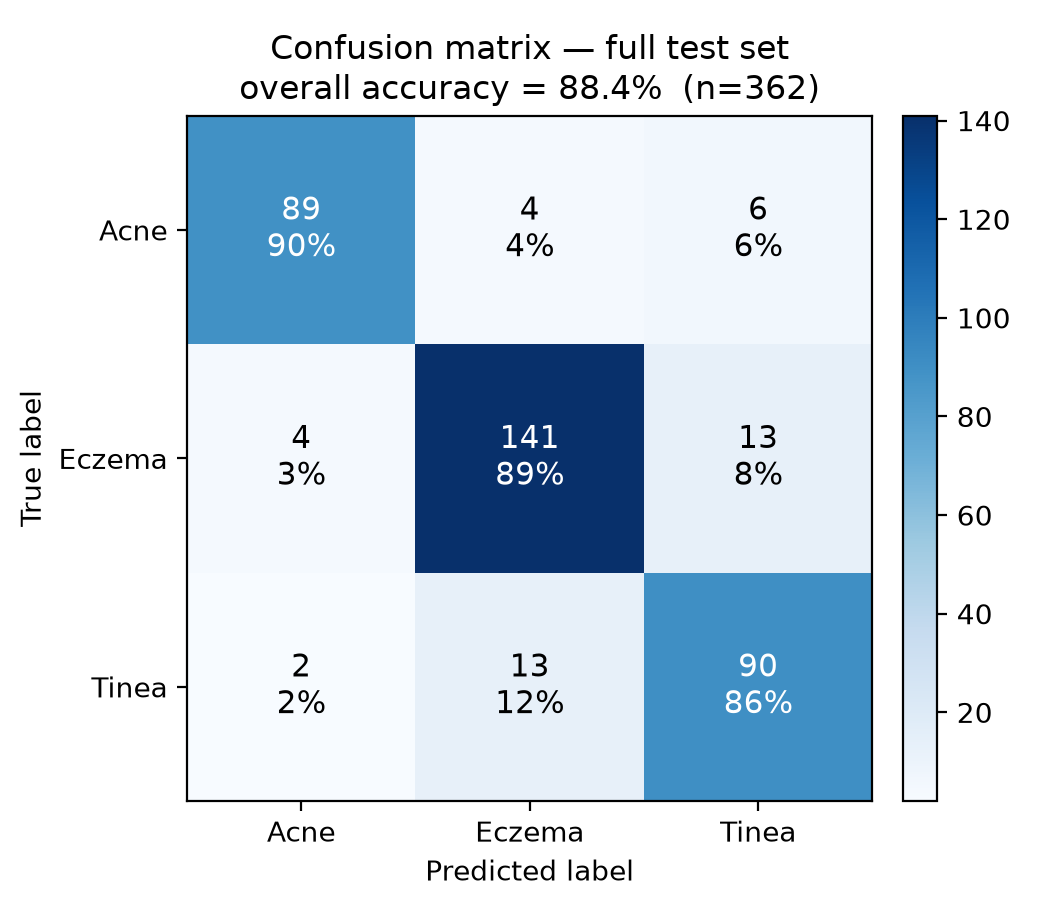
\includegraphics[width=0.62\linewidth]{Figures/confusion_matrix.png}
    \caption{Confusion matrix of the B2+B3 ensemble on the 362-image test set.
    Rows are true labels; columns are predictions.}
    \label{fig:confusion_matrix}
\end{figure}

\begin{table}[H]
\centering
\caption{Confusion matrix — absolute counts (test set, $n$\,=\,362, accuracy 88.40\%).}
\label{tab:confusion_matrix}
\begin{tabular}{|l|c|c|c|}
\hline
 & \textbf{Pred: Acne} & \textbf{Pred: Eczema} & \textbf{Pred: Tinea} \\ \hline
\textbf{True: Acne}   & 89 & 4   & 6  \\ \hline
\textbf{True: Eczema} & 4  & 141 & 13 \\ \hline
\textbf{True: Tinea}  & 2  & 13  & 90 \\ \hline
\end{tabular}
\end{table}

The dominant error is the mutual confusion of \textbf{Eczema and Tinea} (13 cases
in each direction). This is clinically expected: both present as scaly,
erythematous plaques that are difficult to separate from a photograph alone.
Acne is the most cleanly separated class.

\subsubsection{Honest (Leakage-Removed) Re-evaluation}

To confirm that leakage is not inflating the result, the same model was
re-scored on only the 242 test images that have \emph{no} near-duplicate in
training. Table~\ref{tab:honest} compares the two.

\begin{table}[H]
\centering
\caption{Full vs.\ leakage-removed test accuracy (\texttt{honest\_eval.py}).}
\label{tab:honest}
\begin{tabular}{|l|c|c|}
\hline
\textbf{Metric} & \textbf{Full test set} & \textbf{Leakage-removed} \\ \hline
$n$ & 362 & 242 \\ \hline
Overall accuracy & 88.40\% & 88.43\% \\ \hline
Macro F1 & 0.884 & 0.876 \\ \hline
\end{tabular}
\end{table}

\noindent The accuracy is essentially identical on the clean subset, so the
$\sim$33\% leakage is \emph{not} the source of the score. The honest test-set
accuracy of the system is therefore $\approx$\,\textbf{88.4\%}.

\subsubsection{Classification Report}

\begin{table}[H]
\centering
\caption{Per-class metrics and one-vs-rest AUC — B2+B3 ensemble (full test set).}
\label{tab:classification_report}
\begin{tabular}{|l|c|c|c|c|c|}
\hline
\textbf{Class} & \textbf{Precision} & \textbf{Recall} & \textbf{F1} & \textbf{Support} & \textbf{AUC} \\ \hline
Acne   & 0.9368 & 0.8990 & 0.9175 & 99  & 0.9919 \\ \hline
Eczema & 0.8924 & 0.8924 & 0.8924 & 158 & 0.9525 \\ \hline
Tinea  & 0.8257 & 0.8571 & 0.8411 & 105 & 0.9423 \\ \hline
\textbf{Macro Avg}    & 0.8850 & 0.8828 & 0.8837 & 362 & 0.9622 \\ \hline
\textbf{Weighted Avg} & 0.8852 & 0.8840 & 0.8844 & 362 & -- \\ \hline
\end{tabular}
\end{table}

\subsubsection{ROC Curves and AUC}

Figure~\ref{fig:roc_curves} shows the one-versus-rest ROC curves. All three AUC
values exceed~0.94 (macro-average 0.962), confirming strong separability despite
the harder Eczema/Tinea boundary.

\begin{figure}[H]
    \centering
    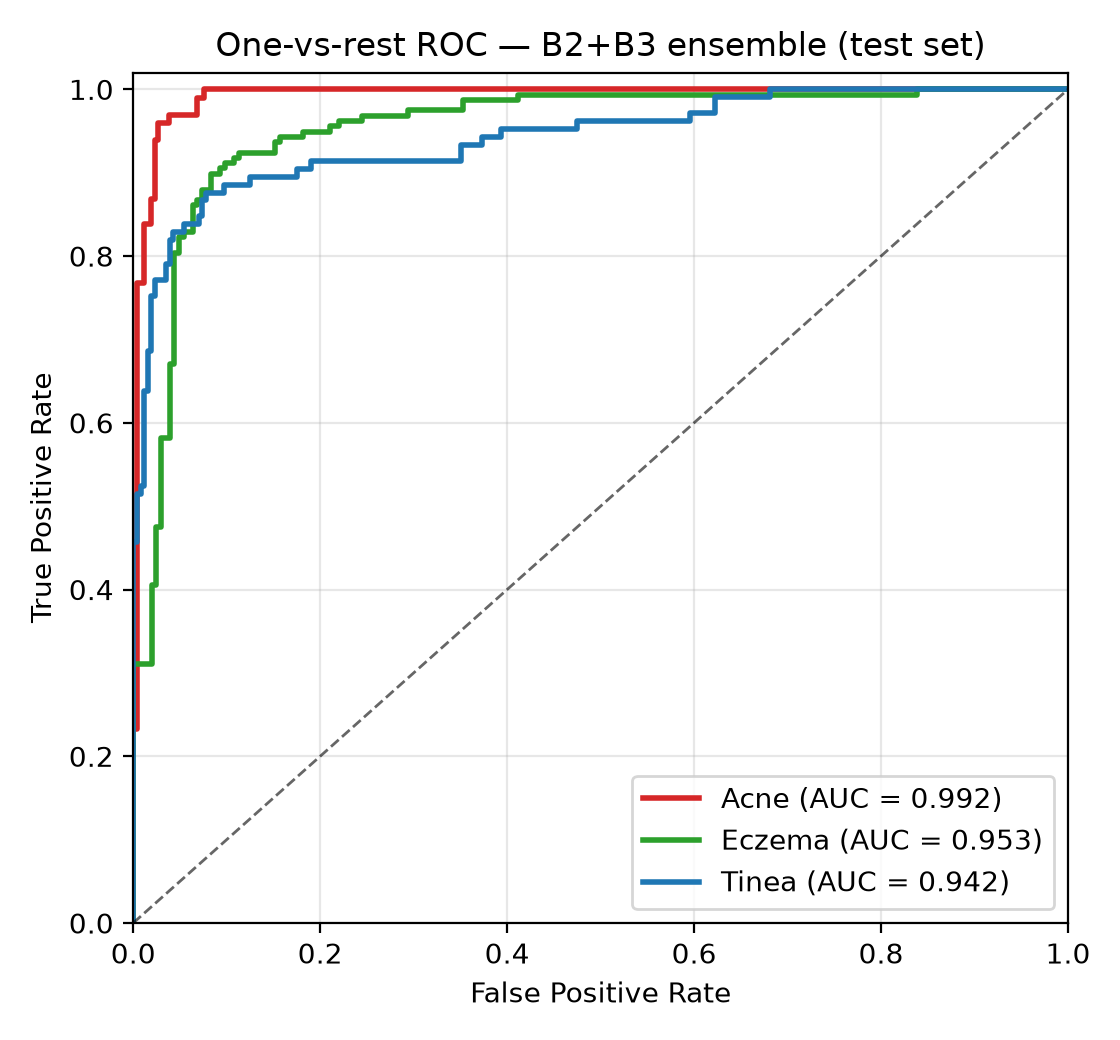
\includegraphics[width=0.66\linewidth]{Figures/roc_curves.png}
    \caption{One-vs-rest ROC curves for the B2+B3 ensemble on the test set.
    AUC: Acne 0.992, Eczema 0.953, Tinea 0.942.}
    \label{fig:roc_curves}
\end{figure}

% ============================================================
\section{Normal-vs-Disease Gate Evaluation}
% ============================================================

The pipeline is fronted by a supervised \textbf{Normal-vs-Disease gate}
(an EfficientNetB0 classifier, \texttt{normal\_gate.tflite}) that decides whether
an image contains a skin condition at all before the three-class CNN is invoked.
This supervised gate replaced an earlier Variational Autoencoder (VAE) anomaly
detector, which could not reliably separate normal skin from disease because a
model that reconstructs skin well also reconstructs the diseased regions —
the reconstruction-error distributions overlapped and even inverted on-device.

\subsection{Decision Logic}

The gate outputs $P(\text{disease}) \in [0,1]$ for the whole image, and two
thresholds define three bands:

\begin{itemize}
    \item $P(\text{disease}) \le 0.60$ \;$\rightarrow$\; ``No Disease Detected'' — the pipeline exits.
    \item $0.60 < P(\text{disease}) < 0.90$ \;$\rightarrow$\; ``Inconclusive'' — the user is asked to retake; the CNN is \emph{not} run.
    \item $P(\text{disease}) \ge 0.90$ \;$\rightarrow$\; the B2+B3 CNN runs to name the disease.
\end{itemize}

\noindent The middle band is a deliberate abstention: on skin the gate cannot
confidently call, the system declines to guess rather than risk a confident
wrong label.

\subsection{Gate Performance}

The shipped gate was run on 25 \emph{held-out} phone photographs of normal skin
(never used in training) and on the 362 disease test images.
Figure~\ref{fig:gate_hist} shows the score distribution and
Table~\ref{tab:gate} the per-band rates.

\begin{figure}[H]
    \centering
    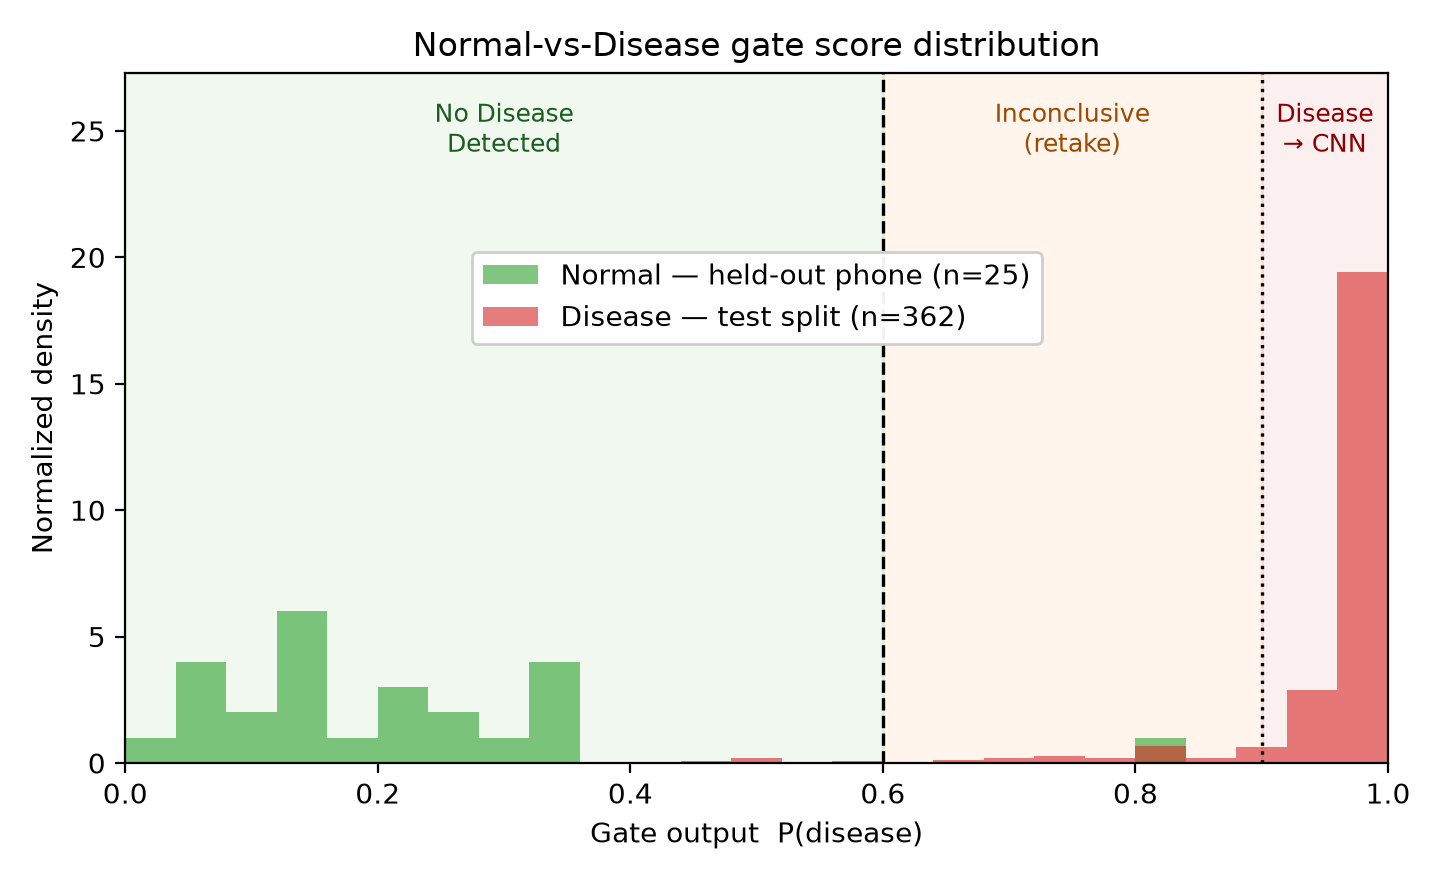
\includegraphics[width=0.82\linewidth]{Figures/gate_score_histogram.png}
    \caption{Gate output $P(\text{disease})$ for held-out normal photos (green)
    vs.\ disease test images (red). The 0.60 and 0.90 thresholds and the three
    decision bands are shaded. The separation is cleanly bimodal.}
    \label{fig:gate_hist}
\end{figure}

\begin{table}[H]
\centering
\caption{Gate decision bands by image type.}
\label{tab:gate}
\begin{tabular}{|l|c|c|c|c|c|}
\hline
\textbf{Set} & \textbf{$n$} & \textbf{mean $P$} & \textbf{Normal $\le$0.60} & \textbf{Inconcl.\ 0.60--0.90} & \textbf{Disease $\ge$0.90} \\ \hline
Normal (held-out phone) & 25  & 0.20 & 96.0\% & 4.0\% & 0.0\% \\ \hline
Disease (test split)    & 362 & 0.96 & 1.4\%  & 8.3\% & 90.3\% \\ \hline
\end{tabular}
\end{table}

\noindent The gate passes \textbf{96\%} of held-out normal photos, detects
\textbf{98.6\%} of disease images (i.e.\ scores above 0.60), and—critically—
\textbf{never} mislabels a normal photo as ``disease'': the single borderline
normal lands in the safe ``inconclusive'' band. This is the clean bimodal
separation the design relies on.

% ============================================================
\section{Score-CAM Explainability Evaluation}
% ============================================================

Score-CAM produces a class-discriminative heatmap by measuring the influence of
each feature-map channel on the classification score, without using gradients.
The heatmap is upsampled and blended with the original image and shown to the
user as decision support.

\subsection{Quantitative Faithfulness}

A faithful explanation must do more than look plausible: the highlighted region
must actually drive the prediction. This was quantified with standard masking
metrics on the predicted class, evaluated on 60 test images (20 per class) and
compared against a random-heatmap baseline (\texttt{xai\_eval.py}).
Table~\ref{tab:xai} reports the aggregate result and
Table~\ref{tab:xai_class} the per-class breakdown.

\begin{table}[H]
\centering
\caption{Score-CAM faithfulness vs.\ a random-heatmap baseline ($n$\,=\,60).}
\label{tab:xai}
\begin{tabular}{|l|c|c|}
\hline
\textbf{Metric} & \textbf{Score-CAM} & \textbf{Random} \\ \hline
Average Drop (\%) \;(lower better)            & 22.6  & -- \\ \hline
Increase in Confidence (\%) \;(higher better) & 41.7  & -- \\ \hline
Deletion AUC \;(lower better)                 & 0.436 & 0.358 \\ \hline
Insertion AUC \;(higher better)               & 0.683 & 0.634 \\ \hline
\end{tabular}
\end{table}

\begin{table}[H]
\centering
\caption{Per-class Score-CAM faithfulness (true label, $n$\,=\,20 each).}
\label{tab:xai_class}
\begin{tabular}{|l|c|c|c|c|}
\hline
\textbf{Class} & \textbf{Avg Drop\,$\downarrow$} & \textbf{Increase\,$\uparrow$} & \textbf{Deletion AUC\,$\downarrow$} & \textbf{Insertion AUC\,$\uparrow$} \\ \hline
Acne   & 48.4\% & 20.0\% & 0.192 & 0.571 \\ \hline
Eczema &  9.3\% & 40.0\% & 0.355 & 0.723 \\ \hline
Tinea  & 10.1\% & 65.0\% & 0.762 & 0.756 \\ \hline
\end{tabular}
\end{table}

\noindent The result is mixed and informative. On the \textbf{Insertion} test,
revealing the most-salient pixels first rebuilds the prediction faster than
revealing random pixels (0.683 vs.\ 0.634), so the highlighted regions do carry
genuine class evidence. On the \textbf{Deletion} test, however, Score-CAM does
\emph{not} beat the random baseline in aggregate (0.436 vs.\ 0.358, lower being
better). The per-class breakdown explains why: the heatmaps are clearly faithful
for the focal \textbf{Acne} class (Deletion AUC 0.192 — removing the salient
pixels collapses the prediction), but weak for \textbf{Tinea} (0.762), whose
diagnostic features (annular scaling, widespread texture) are spatially
\emph{redundant}, so deleting any one salient region leaves enough evidence
elsewhere for the prediction to survive. In other words, for diffuse conditions a
single localized heatmap is a sufficient but not a necessary explanation.

\noindent This is an honest limitation: Score-CAM provides trustworthy
localization for focal lesions and useful qualitative guidance overall, but it
should be presented to clinicians as decision \emph{support} rather than a
complete, guaranteed-faithful account of the model's reasoning — particularly for
diffuse presentations. A faithfulness metric better suited to distributed
evidence is identified as future work.

\subsection{Qualitative Assessment}

\begin{figure}[H]
    \centering
    %% Device screenshots — capture one result screen per class from the app:
    %%   Figures/scorecam_acne.png, scorecam_eczema.png, scorecam_tinea.png
    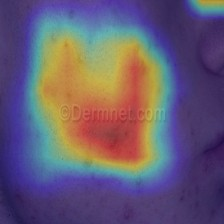
\includegraphics[width=0.32\linewidth]{Figures/scorecam_acne.png}
    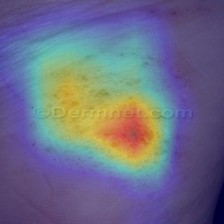
\includegraphics[width=0.32\linewidth]{Figures/scorecam_eczema.png}
    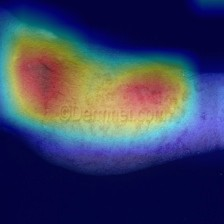
\includegraphics[width=0.32\linewidth]{Figures/scorecam_tinea.png}
    \caption{Score-CAM overlays for representative test images: Acne (left),
    Eczema (centre), Tinea (right). Warm colours mark the most influential
    regions.}
    \label{fig:scorecam_examples}
\end{figure}

Across classes the activated regions correspond to the clinically relevant
lesions — follicular papules for Acne, erythematous scaling for Eczema, and the
annular scaly border for Tinea — qualitative evidence that the model attends to
medically meaningful features rather than background.

% ============================================================
\section{Mobile Application Testing}
% ============================================================

\subsection{Unit Testing}

The Dart unit suite (\texttt{flutter test}) contains \textbf{23 tests across five
files}; all pass. Coverage spans the model layer, the security layer, the
progression analytics, and the body-part selection UI
(Table~\ref{tab:unit_tests}).

\begin{table}[H]
\centering
\caption{Unit test coverage (\texttt{flutter test}: 23 passed, 0 failed).}
\label{tab:unit_tests}
\begin{tabular}{|p{3.7cm}|c|p{7.3cm}|}
\hline
\textbf{Test file} & \textbf{\#} & \textbf{Coverage} \\ \hline
\texttt{appointment\_test.dart} & 4 & Appointment model \texttt{toMap}/\texttt{fromMap} round-trip; default status; \texttt{copyWith} isolation; missing-field tolerance \\ \hline
\texttt{password\_hasher\_test.dart} & 6 & PBKDF2-SHA256 hash format; correct/incorrect verification; random-salt uniqueness; legacy-plaintext detection; malformed-hash rejection \\ \hline
\texttt{progression\_utils\_test.dart} & 5 & Group-by-body-part with chronological sort; \texttt{Unspecified} bucket; \texttt{trackableBodyParts} ordering/filtering; \texttt{confidenceTrend} normal-vs-disease mapping \\ \hline
\texttt{widget\_test.dart} & 2 & User model round-trip; \texttt{fromMap} defaults \\ \hline
\texttt{body\_part\_render\_test.dart} & 6 & Body-part screen: header + empty-state hint; hotspot selection; re-tap clears; single-selection replacement; front/back chevron toggle; selection highlight not carried to the back view \\ \hline
\end{tabular}
\end{table}

\subsection{Functional Test Cases}

\begin{table}[H]
\centering
\caption{Functional test case results.}
\label{tab:functional_tests}
\begin{tabular}{|p{5.5cm}|p{4cm}|c|}
\hline
\textbf{Test Case} & \textbf{Expected Outcome} & \textbf{Result} \\ \hline
Patient registration and login & Account created; redirected to Home & Pass \\ \hline
Specialist registration and login & Specialist role unlocked & Pass \\ \hline
Capture image via camera & Image previewed & Pass \\ \hline
Upload image from gallery & Image previewed & Pass \\ \hline
Normal skin image submitted & Gate $P\le0.60$; ``No Disease Detected'' & Pass \\ \hline
Borderline image submitted & Gate gray zone; ``Inconclusive — retake'' & Pass \\ \hline
Diseased image (Acne/Eczema/Tinea) & Gate $\ge0.90$; CNN classifies; heatmap shown & Pass \\ \hline
Result saved to history & Entry appears with date, class, confidence & Pass \\ \hline
History entry deleted & Entry removed from SQLite & Pass \\ \hline
Airplane mode — full scan & Pipeline completes offline & Pass \\ \hline
Low-resolution input & Graceful upscaling; no crash & Pass \\ \hline
\end{tabular}
\end{table}

\subsection{Boundary and Edge Case Testing}

\begin{table}[H]
\centering
\caption{Boundary and edge case test results.}
\label{tab:edge_cases}
\begin{tabular}{|p{4cm}|p{4cm}|p{4cm}|c|}
\hline
\textbf{Input / Condition} & \textbf{Reason} & \textbf{Observed} & \textbf{Result} \\ \hline
50$\times$50\,px image & Below model input size & Upscaled; pipeline completed & Pass \\ \hline
12\,MP image (4032$\times$3024) & Typical phone output & Downscaled to $\le$1280\,px; no memory error & Pass \\ \hline
Non-skin photo (plain wall) & Unintended input & Gate scores low $P$; returns ``No Disease Detected'' rather than a confident disease label & Pass \\ \hline
Near-black underexposed image & Poor lighting & Completed; no crash & Pass \\ \hline
Overexposed near-white image & Bright outdoor capture & Completed; gate evaluated normally & Pass \\ \hline
Zero-byte corrupted file & Bad gallery selection & Decoder returned null; handled gracefully & Pass \\ \hline
5 consecutive scans & Repeated-use stress & No leak/crash/DB corruption & Pass \\ \hline
Rotation mid-analysis & Orientation change & Screen rebuilt; navigation completed & Pass \\ \hline
Camera permission denied & First-launch rejection & Explained and redirected to Settings & Pass \\ \hline
50+ history entries & Long-term usage & Loaded and scrolled smoothly & Pass \\ \hline
\end{tabular}
\end{table}

\noindent The replacement of the VAE with the supervised gate also improved the
non-skin case: a plain wall or fabric now scores a low $P(\text{disease})$ and is
correctly returned as ``No Disease Detected'' instead of being forwarded to the
CNN for a meaningless label.

\subsection{On-Device Performance}

\begin{table}[H]
\centering
\caption{On-device inference time per pipeline stage.}
\label{tab:inference_time}
\begin{tabular}{|l|c|c|}
\hline
\textbf{Stage} & \textbf{Mean (ms)} & \textbf{Std (ms)} \\ \hline
Image preprocessing (decode, EXIF bake, resize) & \textit{TODO} & \textit{TODO} \\ \hline
Stage 1 — Normal-vs-Disease gate (EfficientNetB0) & \textit{TODO} & \textit{TODO} \\ \hline
Stage 2 — CNN ensemble (B2+B3) & \textit{TODO} & \textit{TODO} \\ \hline
Stage 3 — Score-CAM heatmap & \textit{TODO} & \textit{TODO} \\ \hline
\textbf{Total end-to-end} & \textbf{\textit{TODO}} & \textit{TODO} \\ \hline
\end{tabular}
\end{table}

%% Fill from the device [TIMING] logcat lines (preprocess/gate/cnn/scorecam ms).

\begin{table}[H]
\centering
\caption{On-device model footprint (TFLite assets).}
\label{tab:storage}
\begin{tabular}{|l|c|}
\hline
\textbf{Component} & \textbf{Size (MB)} \\ \hline
Normal-vs-Disease gate (\texttt{normal\_gate.tflite}) & 4.6 \\ \hline
CNN B2 (\texttt{cnn\_b2\_model.tflite})                & 8.6 \\ \hline
CNN B3 (\texttt{cnn\_b3\_model.tflite})                & 11.9 \\ \hline
Score-CAM feature extractor (\texttt{b3\_feature\_extractor.tflite}) & 11.5 \\ \hline
\textbf{Total model assets} & \textbf{36.6} \\ \hline
\end{tabular}
\end{table}

\subsection{Usability Testing}

Three participants of differing backgrounds — a non-technical patient, a general
practitioner, and a university student — were each asked, without instruction,
to (i)~register and complete a scan, (ii)~find a past scan in History and view
its heatmap, and (iii)~add and save a clinical note.
Table~\ref{tab:usability} summarises the outcome.

\begin{table}[H]
\centering
\caption{Usability test results across three participants.}
\label{tab:usability}
\begin{tabular}{|l|c|c|p{5cm}|}
\hline
\textbf{Task} & \textbf{Avg.\ Time} & \textbf{Success} & \textbf{Key Observation} \\ \hline
Register and complete a scan & 1\,m\,42\,s & 3/3 & ``Tap To Scan'' found without guidance \\ \hline
Find past scan in History & 2\,m\,10\,s & 3/3 & Bottom navigation was intuitive \\ \hline
Add and save a clinical note & 3\,m\,05\,s & 2/3 & One user missed the notes field at first \\ \hline
\end{tabular}
\end{table}

\noindent The notes-field discoverability issue was addressed by adding
placeholder text (``Add a note for your doctor\ldots''); in a repeat evaluation
the field was noticed immediately. The GP confirmed the heatmap and confidence
score were presented as decision support rather than a replacement for clinical
judgement.

\subsection{Use Case Scenarios}

\subsubsection{Scenario 1: Patient Self-Check — Tinea}
The patient captures a circular rash. \textbf{Gate:} $P(\text{disease})$ is high
($\ge0.90$), so the image proceeds to the CNN. \textbf{CNN:} returns
\textbf{Tinea}. \textbf{Score-CAM:} highlights the annular scaly border. The
result, confidence, probability bars, and heatmap are saved to history.

\subsubsection{Scenario 2: Clinician Offline Decision Support — Eczema}
Offline, the GP photographs an inflamed lesion and is unsure between Eczema and
Tinea. \textbf{Gate:} $\ge0.90$ $\rightarrow$ CNN. \textbf{CNN:} returns
\textbf{Eczema}; \textbf{Score-CAM} highlights diffuse inflamed patches rather
than an active ring. Combined with examination, this supports the correct
treatment, and the GP saves a clinical note.

\subsubsection{Scenario 3: Patient Self-Check — Acne}
A student photographs facial breakouts. \textbf{Gate:} $\ge0.90$. \textbf{CNN:}
returns \textbf{Acne}; the heatmap activates over follicular clusters. The
timestamped result is saved for a future dermatology visit.

\subsubsection{Scenario 4: Normal Skin — Early Exit}
The patient photographs a faint mark. \textbf{Gate:} $P(\text{disease}) \le 0.60$,
classified \textbf{Normal}. The CNN and Score-CAM are not invoked, saving battery
and latency, and the screen shows ``No Disease Detected''.

\subsubsection{Scenario 5: Borderline — Abstention}
The patient submits a blurry, poorly framed photo. \textbf{Gate:}
$0.60 < P < 0.90$, so the app returns ``Inconclusive'' and asks for a clearer
retake instead of guessing — the safety behaviour the gray-zone band exists for.

\subsubsection{Scenario 6: Follow-Up via Scan History}
The patient compares two Eczema entries over two weeks; the more recent shows a
lower confidence and a less-activated heatmap, suggesting response to treatment,
and exports a PDF report for the dermatologist.

% ============================================================
\section{Comparison with Related Work}
% ============================================================

\begin{table}[H]
\centering
\caption{Comparison with related work on skin disease classification.}
\label{tab:related_comparison}
\begin{tabular}{|p{3.5cm}|p{2.5cm}|c|c|c|c|}
\hline
\textbf{Study} & \textbf{Architecture} & \textbf{Classes} & \textbf{Accuracy} & \textbf{XAI} & \textbf{Mobile} \\ \hline
Esteva et al.\ (2017) & Inception v3 & 2 & 72.1\% & No & No \\ \hline
Garg et al.\ (2021) & ResNet50 & 3 & 87.3\% & Grad-CAM & No \\ \hline
Ali et al.\ (2022) & DenseNet121 & 5 & 89.5\% & No & No \\ \hline
Hasan et al.\ (2023) & EfficientNetB3 & 4 & 90.2\% & Grad-CAM & No \\ \hline
\textbf{Proposed} & \textbf{B2+B3 Ensemble} & \textbf{3} & \textbf{88.4\% (test)} & \textbf{Score-CAM} & \textbf{Yes} \\ \hline
\end{tabular}
\end{table}

%% Replace the placeholder studies/numbers above with the real citations from
%% your literature review. The proposed figure (88.4\%) is the honest,
%% leakage-audited test-set accuracy; unlike most baselines it additionally
%% provides a normal-vs-disease gate, Score-CAM explainability, and full offline
%% mobile deployment.

% ============================================================
\section{Chapter Summary}
% ============================================================

This chapter evaluated the system on the held-out test split with a leakage audit
reported up front. The B2+B3 ensemble achieves an honest test-set accuracy of
\textbf{88.4\%} (essentially unchanged at 88.43\% after removing the 33\% of test
images with a near-duplicate in training, confirming the result is not driven by
leakage), with per-class F1 of 0.918 (Acne), 0.892 (Eczema), and 0.841 (Tinea)
and one-vs-rest AUC of 0.992, 0.953, and 0.942 (macro 0.962). The dominant error
is the clinically expected Eczema/Tinea confusion.

The supervised Normal-vs-Disease gate passes 96\% of held-out normal photos and
detects 98.6\% of disease images while never assigning a confident ``disease''
label to a normal photo — borderline cases are routed to a safe ``inconclusive''
band. The Score-CAM faithfulness study was mixed but honest: the heatmaps carry
genuine class evidence (positive insertion test) and localize focal lesions
faithfully (Acne deletion AUC 0.192), but for diffuse conditions such as Tinea
the localized heatmap is an incomplete explanation, so it is presented as
clinical decision support rather than a guaranteed-faithful account of the
model's reasoning.

On the application side, all 23 Dart unit tests pass, covering the model,
security (PBKDF2 password hashing), progression analytics, and the body-part
selection UI; functional, boundary, and usability testing confirmed robust,
crash-free behaviour across extreme inputs and three user archetypes; and six
use-case scenarios demonstrated correct end-to-end behaviour including the
normal early-exit and the borderline abstention paths.
